%%%%%%%%%%%%%%%%%%%%%%%%%%%%%%%%%%%%%%%%%%%%%%%%%%%%%%%%%%%%%%%%%%%%%%%%%%%%%%%%
%2345678901234567890123456789012345678901234567890123456789012345678901234567890
%        1         2         3         4         5         6         7         8

\documentclass[letterpaper, 10 pt, conference]{ieeeconf}  % Comment this line out
                                                          % if you need a4paper
%\documentclass[a4paper, 10pt, conference]{ieeeconf}      % Use this line for a4
                                                          % paper

\IEEEoverridecommandlockouts                              % This command is only
                                                          % needed if you want to
                                                          % use the \thanks command
\overrideIEEEmargins
% See the \addtolength command later in the file to balance the column lengths
% on the last page of the document



% The following packages can be found on http:\\www.ctan.org
%\usepackage{graphics} % for pdf, bitmapped graphics files
%\usepackage{epsfig} % for postscript graphics files
%\usepackage{mathptmx} % assumes new font selection scheme installed
%\usepackage{times} % assumes new font selection scheme installed
%\usepackage{amsmath} % assumes amsmath package installed
%\usepackage{amssymb}  % assumes amsmath package installed
\usepackage{graphicx}

\title{\LARGE \bf
CS4047: In-Course Assessment
}

%\author{ \parbox{3 in}{\centering Huibert Kwakernaak*
%         \thanks{*Use the $\backslash$thanks command to put information here}\\
%         Faculty of Electrical Engineering, Mathematics and Computer Science\\
%         University of Twente\\
%         7500 AE Enschede, The Netherlands\\
%         {\tt\small h.kwakernaak@autsubmit.com}}
%         \hspace*{ 0.5 in}
%         \parbox{3 in}{ \centering Pradeep Misra**
%         \thanks{**The footnote marks may be inserted manually}\\
%        Department of Electrical Engineering \\
%         Wright State University\\
%         Dayton, OH 45435, USA\\
%         {\tt\small pmisra@cs.wright.edu}}
%}

\author{Konrad Dryja - 51552177 \\
  University of Aberdeen \\
  \today% <-this % stops a space
}


\begin{document}



\maketitle
\thispagestyle{empty}
\pagestyle{empty}


%%%%%%%%%%%%%%%%%%%%%%%%%%%%%%%%%%%%%%%%%%%%%%%%%%%%%%%%%%%%%%%%%%%%%%%%%%%%%%%%
\begin{abstract}

  In this paper I present how Artificial Neural Networks and Aritiicial Immune Systems can be useful for companies handling large amount of data or financial information and how those methods can enhance the ongoing operations. I also provide a critical evaluation on each of the techniques and showcase a possibility of combinations. The report closes with reflection on the direction of bio-inspired computing and argues that it can be a very important aspect of financial modelling.

\end{abstract}


%%%%%%%%%%%%%%%%%%%%%%%%%%%%%%%%%%%%%%%%%%%%%%%%%%%%%%%%%%%%%%%%%%%%%%%%%%%%%%%%
\section{INTRODUCTION}

Bio-inspired computing is an ever-expanding area within computer science attempting to apply concepts that we observe in nature and in living organisms to modern algorithms in order to improve their efficiency and accuracy. The combination of efforts by scientists from different departments - such as biology (Genetic Algorithms) or sociology (Particle Swarm Optimisation) - enabled current techniques to learn from their mistakes and adapt to the changing circumstances \& environment. I strongly believe that introduction of such methods into a financial or trading company would help them tackle problems such as stock prediction \cite{gunasekaran2011evaluation} or improving the current Machine Learning efforts - with the ultimate target of increasing the profit potential. In this report, I would like to bring the attention to two of the most common approaches: Artificial Immune Systems and Artificial Neural Networks, where I will explain the potential application and how useful they could be for the business.

\section{ARTIFICIAL IMMUNE SYSTEM}

Artificial Immune System (AIS) draws directly from biology of humans' (and not only) immune systems - organism's first line of defence against unwanted cells or viruses. The exact details and biological explanation behind those concepts can get incredibly complex very quickly, so for the sake of brevity, we can distinguish two major actors: antibodies (held by B / T cells) and antigens (the viruses). The main goal of antibodies is to identify and destroy to antigens - most importantly, the fight is usually a collective effort of the entire system, rather than of the individual cells. Moreover, one of the crucial concepts that carries over from biology into computing application is "self" and "not-self". The immune system should be able to distinguish between bodies belonging to the organism ("self") and the ones that haven't been recognized and thus should be eliminated ("not-self"). Finally, the detection itself is performed either via Clonal Selection or Negative Selection. The former is based on cloning and mutating the bodies with the highest affinity and the later eliminates the bodies not fulfilling determined criteria (e.g., affinity, often presented as Euclidean distance to the nearest antibody).

\subsection{Applications}
One of the more beneficial examples to our business would certainly be stock prediction. Gunasekaran et al. \cite{gunasekaran2011evaluation} presented an experiment where AIS was deployed to measure the trends and fluctuations on Bombay stock exchange. By feeding data for the year of 2009, the scientists were able to predict with a high accuracy the SENSEX Index for the year of 2010 (Root Mean Square Error of 103.106). While constructing the model, various indicators were used, such as Money Flow Index or Simple Moving Average. The study was researching the ultimate error difference between application of AIS and ANN - the former having achieved better results. Figure \ref{fig:stock} shows the exact difference between the actual SENSEX index for Bombai stock exchange, index predicted by AIS and index predicted by ANN. \newline
\begin{figure}[h!]
  \centering
  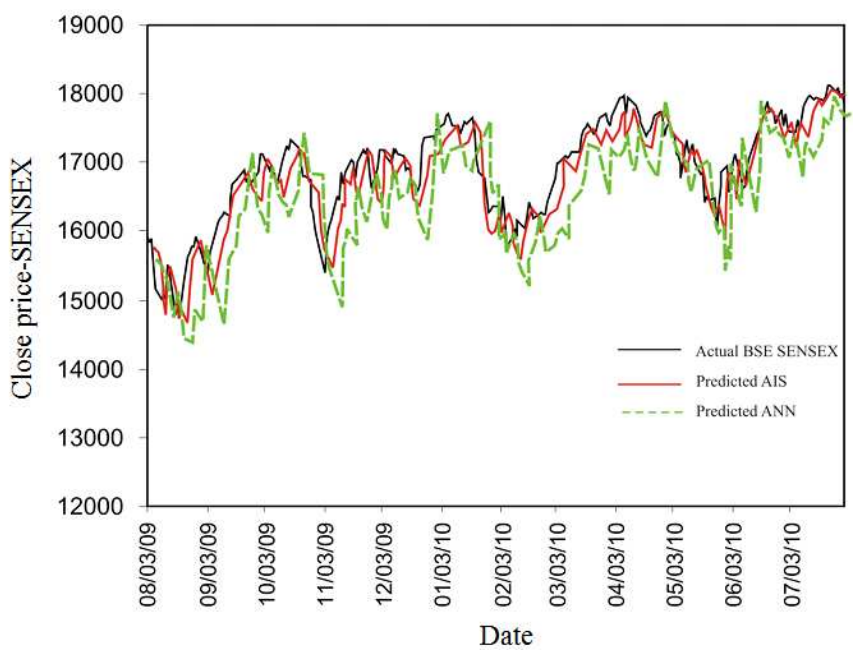
\includegraphics[width=0.4\textwidth]{graph}
  \caption{Comparison of AIS and ANN for stock prediction \cite{gunasekaran2011evaluation}}
  \label{fig:stock}
\end{figure}
Brabazon et al. \cite{brabazon2006biologically} also describes how Negative Selection can be used to determine set of companies that are due to fail and which ones will remain stable. In that particular scenario, "self" can be defined as healthy companies, whereas detectors would be build up from the historical financial data. Then, through the process of selection based on affinity to the detectors, a new set would be detected. Finally, all companies inside "not-self" set would be determined as failing or about to fail. This again could be utilised during decision process for investments. 


\subsection{Strengths} 
\textbf{Memorization:} important perk of AIS (and especially of Clonal Selection) is the ability of reflecting on past experiences and applying that knowledge for future encounters. \cite{timmis2004overview} Detectors that successfully detected an antigen are rewarded with an increased lifespan or are prioritised during cloning to maintain their parameters. 

\textbf{Ease of application:} the universal nature of AIS makes usage and application to any area or problem incredibly easy, yielding satisfactory results. Depending on whether we're using clonal or negative selection. But this can also be seen as a disadvantage, as described in the next section.

\subsection{Weaknesses}
\textbf{Scalability and coverage:} considering the example showing detection of failing companies - which utilizes the negative selection algorithm - one of the biggest challenges would be to handle the ever-growing set of "self", that is the number of companies is going to keep increasing, thus making this task more and more computationally expensive - as presented in the book \cite{brabazon2006biologically}.

\textbf{Jack-of-All-Trades:} Timmis argues \cite{timmis2004overview} that there is no precise field or application which AIS were designed for. This can be seen as both advantage and disadvantage, as it can be applied to a wider range of problems, but at the same time lack of specialization makes it susceptible to exploring breadth of solutions, rather than their depth. For the majority of those problem spaces there already exists a specialised solution yielding better results than AIS \cite{garrett2005we}.

\section{Artificial Neural Networks}
Artificial Neural Networks (ANN) is a slightly different approach to problem solving, also deriving directly from the behaviour of living organisms. In that particular case, brain is considered. To put the things relatively simple, brain contains roughly 100 billion neurons \cite{lent2012many} - each accepting arbitrary input and activating (i.e. passing the information further) based on pre-determined function. We might not be capable to efficiently run and simulate the whole 100 billion of neurons, but we can introduce a simplified model.

\begin{figure}[h!]
  \centering
  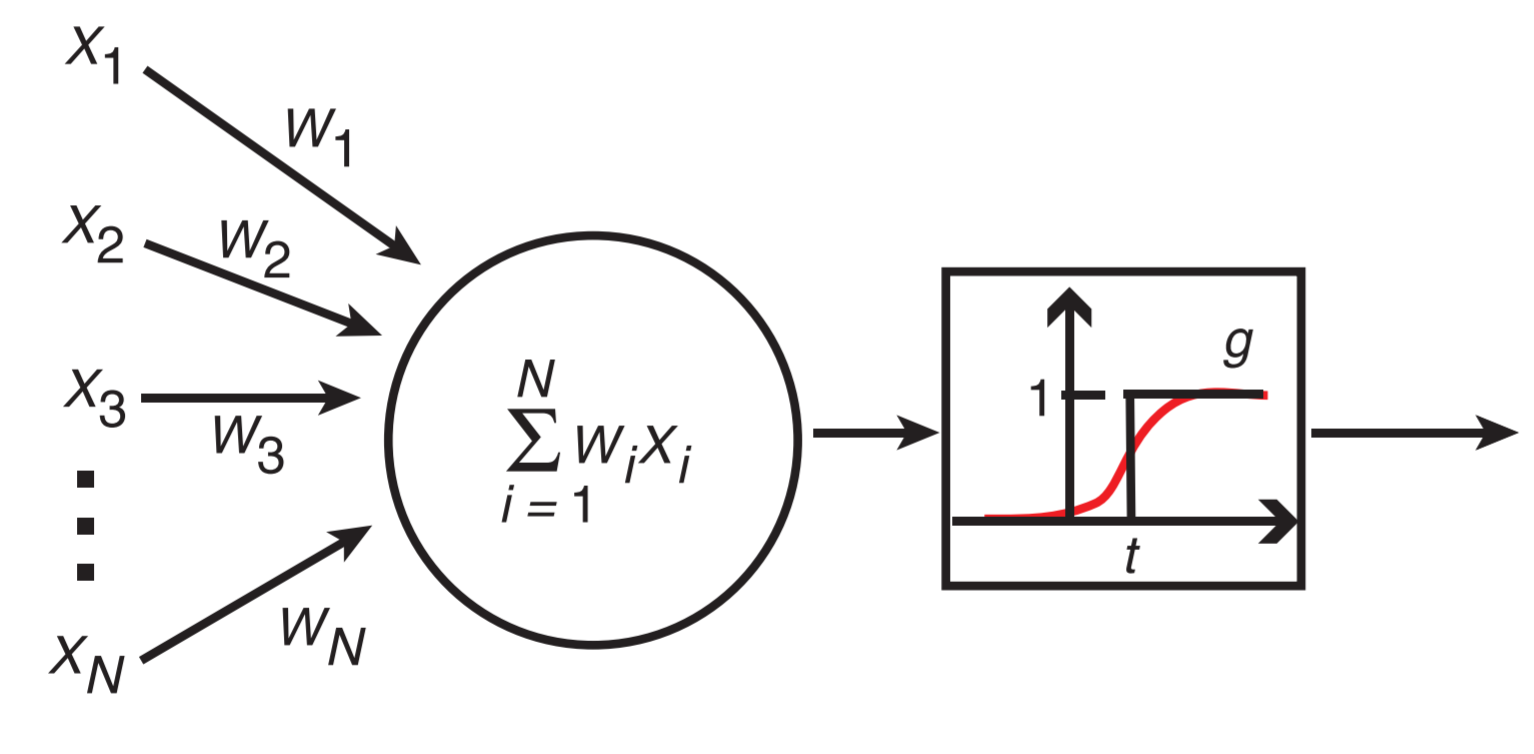
\includegraphics[width=0.4\textwidth]{ann}
  \caption{Example representation of ANN \cite{krogh2008artificial}}
  \label{fig:ann}
\end{figure}

Figure \ref{fig:ann} shows an example Neural Net capable of accepting up to N inputs. Each of them is summed and put into the hidden layer, based on the value of activation function, usually being sigmoid - \(S(x) = \frac{1}{1+e^{-x}}\), where \(x\) is the input multiplied by weight \(w\). The inputs are usually accompanied with constant bias and an extra hidden layer placed after the initial input layer (not shown on the figure).

Furthermore, the network can be further trained by adjusting the weights \(w_n\). For a normal feed-forward neural network it is usually achieved through backpropagation algorithm. After several runs on known data, we can introduce unknown elements and derive the relations.

\subsection{Applications}

When discussing AIS, I presented a use-case where AIS and ANN where faced together in order to predict stock index for Indian market. In fact, the application of neural nets is much wider, consisting of scenarios such as image recognition \cite{tsai1995applying} or further financial modelling. Guresen et al. \cite{guresen2011using} discussed an approach of utilising Multi-Layer Perceptron models for financial forecasting, in particular NASDAQ index. The net was capable of estimating Mean Square Error and Mean Absolute Deviate for future dates, after being trained with past data, hinting at usefulness of the approach in data mining and financial modelling.

\subsection{Strengths}
\textbf{Partial data:} neural nets are designed to handle missing or partial data that's fed into it - once it has been trained for several iterations through backpropagation algorithm. It can also form relations between particular input nodes which haven't been specified before.

\textbf{Fault tolerant:} incomplete or wrong data in one of the inputs does not nullify the results obtained from the network. Those inputs would usually end up with greatly decreased weights, overall limiting their importance - which is achieved through again thanks to backpropagation or other learning algorithms.

\subsection{Weaknesses}
\textbf{Initialization:} the layout and organisation of initial input nodes remains a difficulty when it comes to constructing neural nets. Often slight modification of bias or input weights can result in problems such as overfitting or underfitting. Fortunately, in the next section I'm describing a method of conquering that problem, by combining ANN with Genetic Algorithms (not described in this paper, although yet another biologically derived computation method).

\textbf{Path to the answer:} whereas neural nets work exceptionally well with unknown or partial data, the obtained results very often also remain a subject of interpretation. It is a non-trivial task to establish the exact decision process (such as presenting as Markov Chain) yielding the results.

\section{COMBINATIONS}

As useful as individual methods are, the combination of different bio-inspired computation methods allows for even more powerful and precise machine learning paradigms. One of the most prominent examples being NeuroEvolution of Augmenting Topologies (NEAT) \cite{stanley2002evolving} presented by researches at University of Texas at Austin. The technique combines genetic algorithms along with artificial neural networks, enabling the latter to evolve and change it's layout, such as number and location of particular input nodes in various layers across the network or the weights themselves. That way an ANN can adapt and evolve according to the outside factors. There exists further implementations of neuroevolution algorithms, such as Enforced Subpopulations \cite{ha2015esp}, which hints at the novelty and usefulness of combining various evolutionary paradigms.

\section{CONCLUSIONS}

As I pointed out in the first paragraph, the bio-inspired computing is still a relatively young approach with the possibilities of applying it to many, perhaps previously considered very difficult (such as TSP) problems. Majority of modern machine learning research focus surrounds concepts such as GA or ANN, with great results. Considering the problem space of financial companies (e.g. forecasting with partial data or pattern recognition in analyses), it is a field that could greatly benefit from those technologies and is worth further research \& investments.

\addtolength{\textheight}{-12cm}   % This command serves to balance the column lengths
                                  % on the last page of the document manually. It shortens
                                  % the textheight of the last page by a suitable amount.
                                  % This command does not take effect until the next page
                                  % so it should come on the page before the last. Make
                                  % sure that you do not shorten the textheight too much.

%%%%%%%%%%%%%%%%%%%%%%%%%%%%%%%%%%%%%%%%%%%%%%%%%%%%%%%%%%%%%%%%%%%%%%%%%%%%%%%%



%%%%%%%%%%%%%%%%%%%%%%%%%%%%%%%%%%%%%%%%%%%%%%%%%%%%%%%%%%%%%%%%%%%%%%%%%%%%%%%%



%%%%%%%%%%%%%%%%%%%%%%%%%%%%%%%%%%%%%%%%%%%%%%%%%%%%%%%%%%%%%%%%%%%%%%%%%%%%%%%%

\bibliographystyle{unsrt}
\bibliography{refs}

\end{document}

